% Options for packages loaded elsewhere
\PassOptionsToPackage{unicode}{hyperref}
\PassOptionsToPackage{hyphens}{url}
%
\documentclass[
  11pt,
]{article}
\usepackage{lmodern}
\usepackage{amssymb,amsmath}
\usepackage{ifxetex,ifluatex}
\ifnum 0\ifxetex 1\fi\ifluatex 1\fi=0 % if pdftex
  \usepackage[T1]{fontenc}
  \usepackage[utf8]{inputenc}
  \usepackage{textcomp} % provide euro and other symbols
\else % if luatex or xetex
  \usepackage{unicode-math}
  \defaultfontfeatures{Scale=MatchLowercase}
  \defaultfontfeatures[\rmfamily]{Ligatures=TeX,Scale=1}
\fi
% Use upquote if available, for straight quotes in verbatim environments
\IfFileExists{upquote.sty}{\usepackage{upquote}}{}
\IfFileExists{microtype.sty}{% use microtype if available
  \usepackage[]{microtype}
  \UseMicrotypeSet[protrusion]{basicmath} % disable protrusion for tt fonts
}{}
\makeatletter
\@ifundefined{KOMAClassName}{% if non-KOMA class
  \IfFileExists{parskip.sty}{%
    \usepackage{parskip}
  }{% else
    \setlength{\parindent}{0pt}
    \setlength{\parskip}{6pt plus 2pt minus 1pt}}
}{% if KOMA class
  \KOMAoptions{parskip=half}}
\makeatother
\usepackage{xcolor}
\IfFileExists{xurl.sty}{\usepackage{xurl}}{} % add URL line breaks if available
\IfFileExists{bookmark.sty}{\usepackage{bookmark}}{\usepackage{hyperref}}
\hypersetup{
  pdftitle={From Points to Paychecks: An Exploratory Analysis of NBA Salaries and Performance (2022--23)},
  pdfauthor={Pacific Boys: Marcelino Bautista, Konstantin Khorobrykh, Tim Platz, Da-Wei Lin},
  hidelinks,
  pdfcreator={LaTeX via pandoc}}
\urlstyle{same} % disable monospaced font for URLs
\usepackage[margin=1in]{geometry}
\usepackage{longtable,booktabs}
% Correct order of tables after \paragraph or \subparagraph
\usepackage{etoolbox}
\makeatletter
\patchcmd\longtable{\par}{\if@noskipsec\mbox{}\fi\par}{}{}
\makeatother
% Allow footnotes in longtable head/foot
\IfFileExists{footnotehyper.sty}{\usepackage{footnotehyper}}{\usepackage{footnote}}
\makesavenoteenv{longtable}
\usepackage{graphicx}
\makeatletter
\def\maxwidth{\ifdim\Gin@nat@width>\linewidth\linewidth\else\Gin@nat@width\fi}
\def\maxheight{\ifdim\Gin@nat@height>\textheight\textheight\else\Gin@nat@height\fi}
\makeatother
% Scale images if necessary, so that they will not overflow the page
% margins by default, and it is still possible to overwrite the defaults
% using explicit options in \includegraphics[width, height, ...]{}
\setkeys{Gin}{width=\maxwidth,height=\maxheight,keepaspectratio}
% Set default figure placement to htbp
\makeatletter
\def\fps@figure{htbp}
\makeatother
\setlength{\emergencystretch}{3em} % prevent overfull lines
\providecommand{\tightlist}{%
  \setlength{\itemsep}{0pt}\setlength{\parskip}{0pt}}
\setcounter{secnumdepth}{5}
\usepackage{float}
\usepackage{float}
\usepackage{placeins}
\usepackage{subcaption}
\usepackage{dcolumn}
\usepackage{booktabs}
\usepackage{longtable}
\usepackage{array}
\usepackage{multirow}
\usepackage{wrapfig}
\usepackage{float}
\usepackage{colortbl}
\usepackage{pdflscape}
\usepackage{tabu}
\usepackage{threeparttable}
\usepackage{threeparttablex}
\usepackage[normalem]{ulem}
\usepackage{makecell}
\usepackage{xcolor}

\title{From Points to Paychecks: An Exploratory Analysis of NBA Salaries and Performance (2022--23)}
\author{Pacific Boys: Marcelino Bautista, Konstantin Khorobrykh, Tim Platz, Da-Wei Lin}
\date{2025-04-17}

\begin{document}
\maketitle

{
\setcounter{tocdepth}{2}
\tableofcontents
}
\newpage

\hypertarget{introduction}{%
\section{Introduction}\label{introduction}}

GMs and coaches of NBA teams need to make highstakes decisions when assembling their rosters. With the average NBA player salary topping \$6.62 million for the 2022-23 season ({[}1{]}), the need for data insights is higher than ever. Our goal is to describe how NBA player salaries relate to performance metrics during the 2022-23 \textbf{regular} season. We focus on Points Per Game (PTS) and Minutes Played (MP) as primary predictors, along with other stats like FG, TRB, 3P\%, TOV, WS, AST, and GP. This exploratory analysis will derive actionable insights and enable key stakeholders to make data-driven decisions.

\hypertarget{research-approach}{%
\subsection{Research Approach}\label{research-approach}}

While prior studies use machine learning for salary prediction ({[}2, 3{]}), our Ordinary Least Squares (OLS) regression model prioritizes interpretability
to identify which performance indicators are most descriptively associated (not causal) with compensation. Because this is a team sport, we acknowledge
the presence of dependence among observations and violations of the \textbf{IID} (independent and identically distributed) assumption. However, we proceed with the analysis given our focus on descriptive insights. We will revisit these hypotheses in our conclusion to confirm or refine their validity.

\hypertarget{data-source}{%
\section{Data Source}\label{data-source}}

\begin{itemize}
\tightlist
\item
  \textbf{Primary Source:} \href{https://www.kaggle.com/datasets/jamiewelsh2/nba-player-salaries-2022-23-season/data}{Kaggle NBA Salaries 2022-23}
\item
  \textbf{All-Star Players:} \href{https://www.basketball-reference.com/allstar/NBA_2023.html}{Basketball Reference All-Star 2023}
\item
  \textbf{Years of Experience:} \href{https://www.basketball-reference.com/teams/ATL/2023.html}{Basketball Reference Team Rosters}
\item
  \textbf{Market Size Data:} \href{https://hoop-social.com/nba-team-market-size-rankings/}{NBA Team Market Size Rankings}
\item
  \textbf{Unit:} Individual NBA players
\item
  \textbf{Type:} Cross-sectional snapshot of 2022-23 season
\end{itemize}

\hypertarget{data-wrangling}{%
\section{Data Wrangling}\label{data-wrangling}}

For data wrangling, we began by obtaining the main dataset from Kaggle and iteratively scraping roster data for each team from Basketball Reference. We then added All-Star selections and merged the dataset with market size information. Duplicate entries, primarily from players traded mid-season, were identified and removed. The cleaned data was split into two parts: 30/70 for exploratory data analysis (EDA) and the remainder for confirmatory analysis. The current analysis focuses on the EDA portion.

The raw NBA dataset contains 140 players and 62 variables for the 2022-23 season. After cleaning, the dataset contains 140 active players with valid salary data. We selected 24 key variables including performance metrics, player characteristics, and team information. We understand that Salary is heavily right-skewed, so we created a log-transformed variable (LogSalary) to normalize the distribution. We also created a Box-Cox transformed variable (BoxCoxSalary) with lambda of 0.1455141 to further improve normality.

\hypertarget{operationalization} (3-point shooting percentage), TOV (turnovers), WS (win shares), AST (assists per game), GP (games played)
\item
  \textbf{TVMS:} TV Market Size - represents the size of the team's market
\item
  \textbf{TS\%:} True Shooting Percentage - a measure of shooting efficiency
\end{itemize}

\hypertarget{exploratory-data-analysis}{%
\section{Exploratory Data Analysis}\label{exploratory-data-analysis}}

\hypertarget{salary-distributions-and-star-player-comparison}{%
\subsection{Salary Distributions and Star Player Comparison}\label{salary-distributions-and-star-player-comparison}}

The salary distribution is heavily right-skewed (Figure \ref{fig:salary-distributions}). Applying a log transformation makes the distribution more symmetric and closer to a normal shape (Figure \ref{fig:salary-distributions}). Additionally, rookies are clearly at a disadvantage in terms of salary compared to more experienced players (Figure \ref{fig:salary-distributions}).

\begin{figure}
\centering
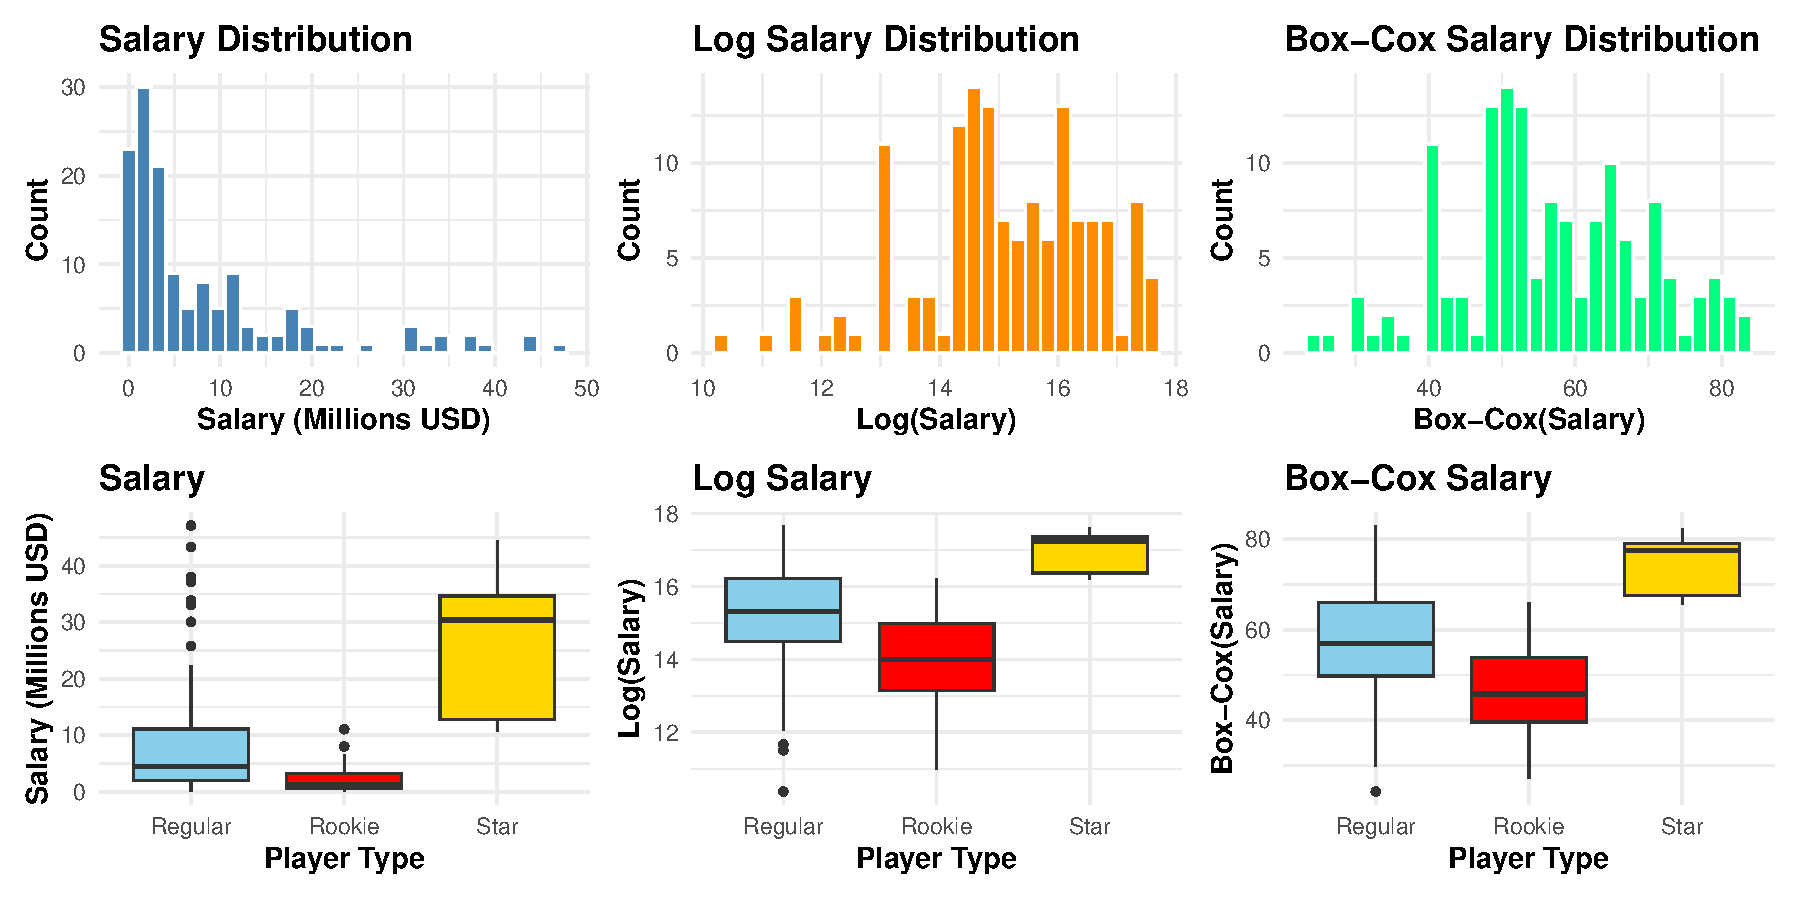
\includegraphics{lab2_report_short_files/figure-latex/salary-distributions-1.pdf}
\caption{\label{fig:salary-distributions}Salary distributions and boxplots by player category}
\end{figure}

\hypertarget{performance-metric-distributions}{%
\subsection{Performance Metric Distributions}\label{performance-metric-distributions}}

PTS and FG are both right-skewed and highly correlated, while MP shows a fairly uniform distribution (Figure \ref{fig:performance-dist}). True Shooting Percentage (TS\%), calculated as TS\% = PTS / (2 * (FGA + 0.44 * FTA))---which integrates scoring from field goals and free throws---tends to cluster around 0.6 regardless of salary (Figure \ref{fig:performance-dist}). Notably, there's an outlier with a TS\% of 0, and interestingly, an individual with a TS\% of 0.8 isn't earning much.

\begin{figure}
\centering
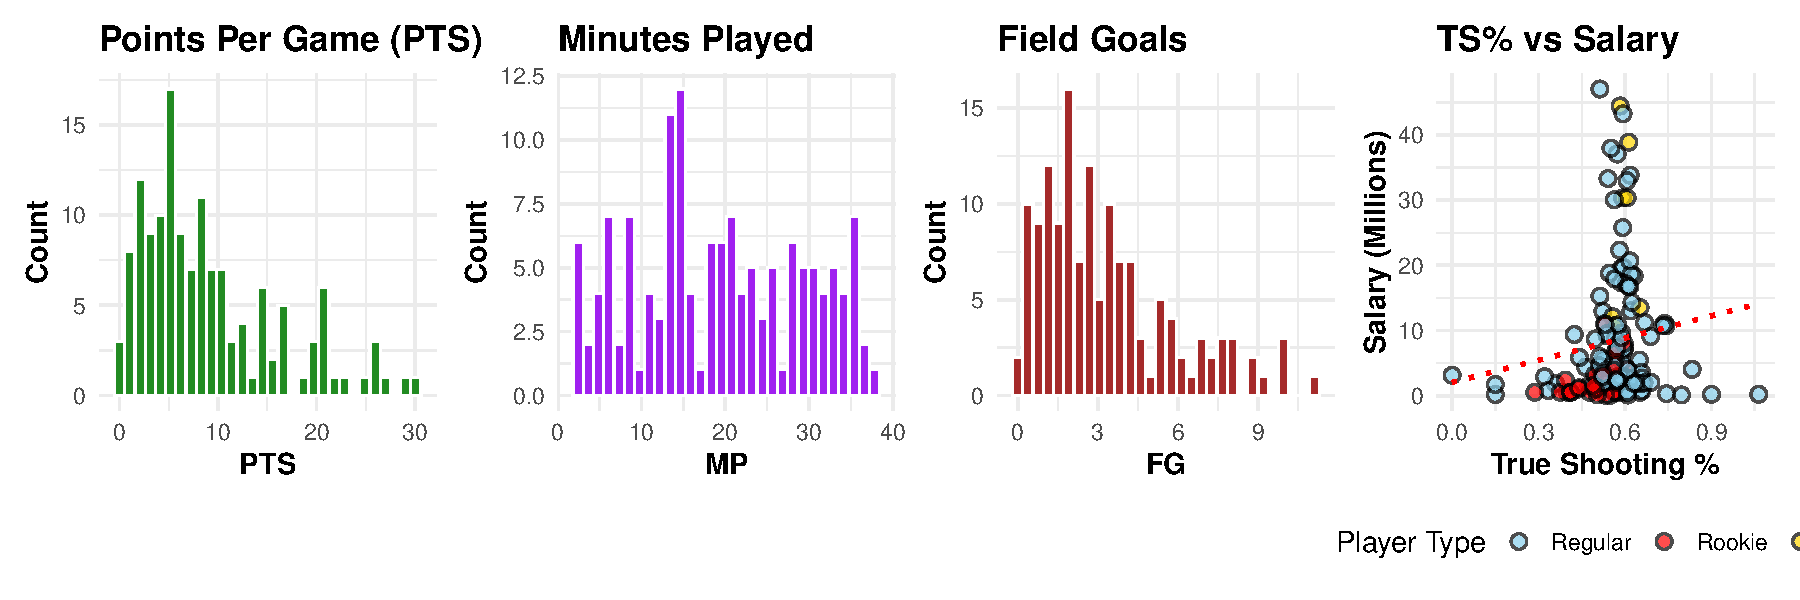
\includegraphics{lab2_report_short_files/figure-latex/performance-dist-1.pdf}
\caption{\label{fig:performance-dist}Performance metric distributions}
\end{figure}

\hypertarget{pairwise-scatter-plots}{%
\subsection{Pairwise Scatter Plots}\label{pairwise-scatter-plots}}

Strong correlations among metrics---such as PTS, MP, WS, and FG---suggest these variables tend to move together (see Appendix Figure \ref{fig:appendix-pairwise}). Additionally, histograms reveal significant right skewness, with TVMS displaying an almost bimodal distribution. Therefore, it's crucial to test for variance inflation factors (VIF) before constructing the models to ensure multicollinearity isn't an issue.

\hypertarget{correlation-matrix}{%
\subsection{Correlation Matrix}\label{correlation-matrix}}

There is a noticeable positive correlation between points (PTS) and other performance metrics such as minutes played (MP), field goals (FG), turnovers (TOV), and win shares (WS) (see Appendix Figure \ref{fig:appendix-corr}). This suggests that market-driven factors captured by TVMS are distinct from on-court performance.

\hypertarget{salary-vs.-key-predictors}{%
\subsection{Salary vs.~Key Predictors}\label{salary-vs.-key-predictors}}

The analysis indicates that performance metrics such as points per game, minutes played, and win shares are strongly correlated with salary, although there are exceptions---such as a rookie with high minutes but a relatively low salary (Appendix Figure \ref{fig:appendix-salary-predictors}). Additionally, salaries tend to rise with years of experience before leveling off, highlighting the impact of tenure and potentially age. There are also clear positional differences; for example, centers and shooting guards tend to have lower median salaries compared to power forwards, who generally command higher median earnings. While there is an observation that players on larger market teams may earn more on average, this relationship appears to be complex and could benefit from further evaluation.

\hypertarget{preliminary-models}{%
\subsection{Preliminary Models}\label{preliminary-models}}

To explore linear relationships between NBA player salaries and various performance metrics, we formulated nine models across three salary transformations. These models assess how different variables influence player compensation during the 2022-23 season.

\hypertarget{model-specifications}{%
\subsubsection{Model Specifications}\label{model-specifications}}

We test three model specifications with three different dependent variables:

\begin{itemize}
\item
  \textbf{Models 1-3}: Raw Salary
\item
  \textbf{Models 4-6}: Log-transformed Salary (LogSalary)
\item
  \textbf{Models 7-9}: Box-Cox transformed Salary (BoxCoxSalary)
\end{itemize}

For each transformation, we test three specifications:

\begin{enumerate}
\def\labelenumi{\arabic{enumi}.}
\item
  \textbf{Basic Model}: Only Points Per Game (PTS)
\item
  \textbf{Performance Model}: PTS, Total Rebounds (TRB), and Assists (AST)
\item
  \textbf{Comprehensive Model}: Performance metrics plus Experience (Exp\_num) and TV Market Size (TVMS)
\end{enumerate}

\hypertarget{collinearity-issues}{%
\subsection{Collinearity Issues}\label{collinearity-issues}}

No collinearity concern with the VIF results (\textless5), see Appendix Table \ref{tab:appendix-vif}.

\hypertarget{heteroscedasticity-robust-standard-error}{%
\subsection{Heteroscedasticity \& Robust Standard Error}\label{heteroscedasticity-robust-standard-error}}

From the fitted value v.s. resudul plot, whereas the first three models exhibit heteroscedasticity, the next six (using log and Box-Cox transformations) are homoscedastic.
These observations are further supported by the Breusch-Pagan test results.
(See Appendix Figure \ref{fig:appendix-hetero} and Appendix Table \ref{tab:appendix-bp}.)

\hypertarget{model-selection-rationale}{%
\subsection{Model Selection Rationale}\label{model-selection-rationale}}

Based on the exploratory models (Appendix~Tables~\ref{tab:appendix-models1}, \ref{tab:appendix-models2}, and \ref{tab:appendix-models3}),
Model 3 (Raw Salary \textasciitilde{} PTS + TRB + AST + Exp\_num + TVMS) with additional selected predictive variables provides improvements in R\^{}2 compared to Model 1 and Model 2.
While log and Box-Cox transformations (Models 4 - 9) successfully decreased heteroscedasticity, they also decreased R\^{}2 and make interpreting coefficients less direct (Appendix Figure \ref{fig:appendix-hetero}).
Model 3 includes key performance metrics, experience, and market size, all showing significance (especially with robust standard errors). Since we can use robust standard errors to address heteroscedasticity, we can still use the raw salary model (Model 3) for interpretability and significance testing.
(Appendix~Table~\ref{tab:appendix-models-robust}). Therefore, we proceed with Model 3 as final model and apply confirmatory dataset to validate our findings.

\hypertarget{confirmatory-analysis-final-model-and-interpretation}{%
\section{Confirmatory Analysis, Final Model, and Interpretation}\label{confirmatory-analysis-final-model-and-interpretation}}

This regression explains about 69\% of the variation in NBA salaries, with scoring (PTS), experience (Expnum), and TV market size (TVMS) emerging as the most influential factors. Specifically, each additional point per game is associated with roughly a \$942~K boost in salary, each year in the league adds about \$1.01~M, and playing in a larger TV market contributes roughly \$642~K, all else held equal. Rebounds and assists do not carry significant weight once scoring is in the model, and visual diagnostics show that predictions align well with actual salaries for most players, though superstar contracts at the high end exhibit greater dispersion.

\hypertarget{model-limitations-and-future-directions-for-improvement}{%
\section{Model Limitations and Future Directions for Improvement}\label{model-limitations-and-future-directions-for-improvement}}

As potential next steps, our model could be refined by incorporating longitudinal data to capture temporal trends in player performance. Additionally, addressing omitted variable bias by including contextual factors---such as changes in league policy, evolving salary structures, the influence of agents, and injury history---may further enhance explanatory power. Stratified modeling, such as developing team-specific or region-specific models, could also improve fit and interpretability. Lastly, exploring nonlinear relationships through the inclusion of quadratic or interaction terms may better capture the complexity inherent in the data.

\begin{figure}[!ht]
  \centering
  %————— LEFT BOX (table) —————
  \begin{minipage}[c]{0.48\textwidth}
    \centering

\begingroup 
\small 
\begin{tabular}{@{\extracolsep{5pt}}lD{.}{.}{-3} } 
\\[-1.8ex]\hline 
\hline \\[-1.8ex] 
 & \multicolumn{1}{c}{\textit{Dependent variable:}} \\ 
\cline{2-2} 
\\[-1.8ex] & \multicolumn{1}{c}{Salary} \\ 
 & \multicolumn{1}{c}{Final Model} \\ 
\hline \\[-1.8ex] 
 PTS & 942,429.500^{***} \\ 
  & (122,593.400) \\ 
  TRB & 225,295.100 \\ 
  & (255,167.000) \\ 
  AST & 19,140.650 \\ 
  & (404,417.300) \\ 
  Exp$_{\text{num}}$ & 1,014,302.000^{***} \\ 
  & (118,423.100) \\ 
  TVMS & 641,778.900^{***} \\ 
  & (222,584.200) \\ 
  Constant & -7,211,120.000^{***} \\ 
  & (848,045.000) \\ 
 \hline \\[-1.8ex] 
Robust p-val: PTS & 0 \\ 
Robust p-val: TRB & 0.378 \\ 
Robust p-val: AST & 0.962 \\ 
Robust p-val: Exp & 0 \\ 
Robust p-val: TVMS & 0.004 \\ 
Observations & \multicolumn{1}{c}{326} \\ 
R$^{2}$ & \multicolumn{1}{c}{0.689} \\ 
Adjusted R$^{2}$ & \multicolumn{1}{c}{0.684} \\ 
Residual Std. Error & \multicolumn{1}{c}{6,083,581.000 (df = 320)} \\ 
F Statistic & \multicolumn{1}{c}{141.784$^{***}$ (df = 5; 320)} \\ 
\hline 
\hline \\[-1.8ex] 
\textit{Note:}  & \multicolumn{1}{r}{$^{*}$p$<$0.1; $^{**}$p$<$0.05; $^{***}$p$<$0.01} \\ 
\end{tabular} 
\endgroup

  \end{minipage}
  \hfill
  %——— RIGHT BOX (plots) ———
  \begin{minipage}[c]{0.48\textwidth}
    \centering

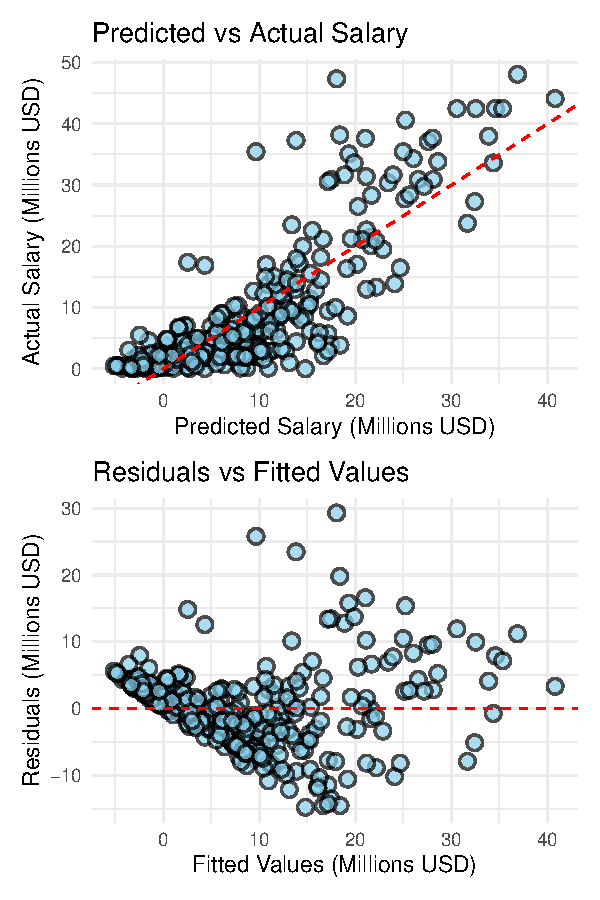
\includegraphics{lab2_report_short_files/figure-latex/plot-side-1.pdf}

  \end{minipage}
  \caption{Final Model Results: (a) Coefficients with robust SE; (b) Predicted vs Actual and residual plots.}
  \label{fig:final_model_side}
\end{figure}

\FloatBarrier

\hypertarget{appendix}{%
\section{Appendix}\label{appendix}}

\hypertarget{fig:appendix-pairwise}{%
\subsection{Pairwise Scatter-Plot Matrix}\label{fig:appendix-pairwise}}

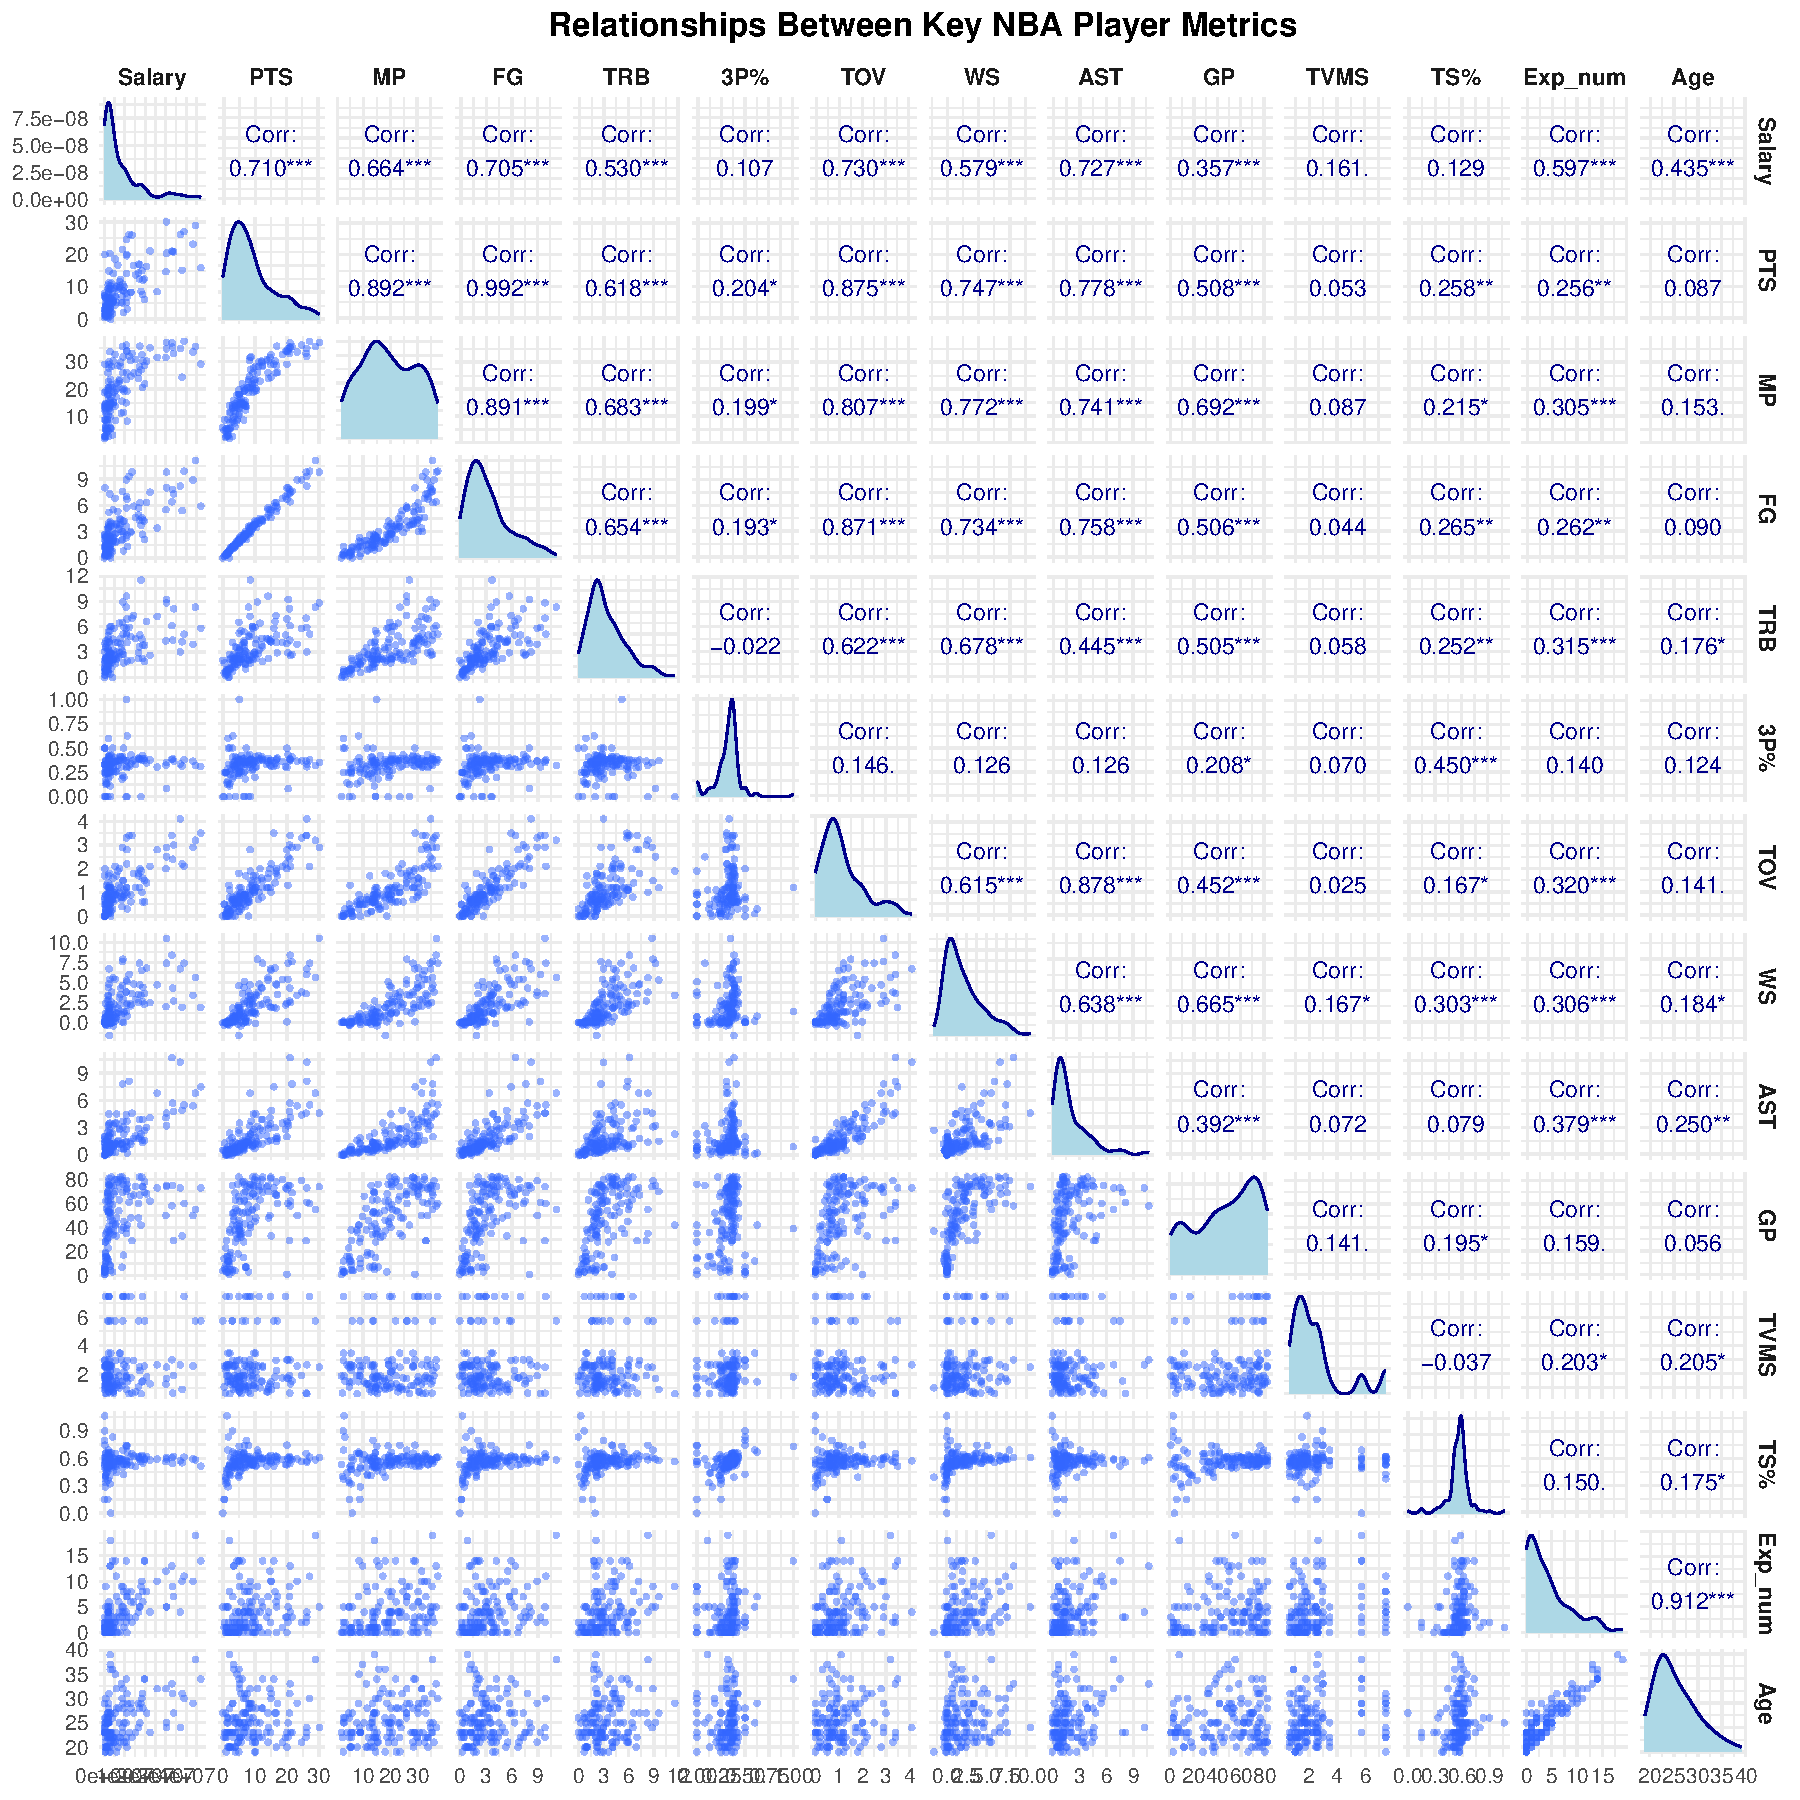
\includegraphics{lab2_report_short_files/figure-latex/appendix-pairwise-scatter-1.pdf}
\FloatBarrier

\hypertarget{fig:appendix-corr}{%
\subsection{Correlation Matrix}\label{fig:appendix-corr}}

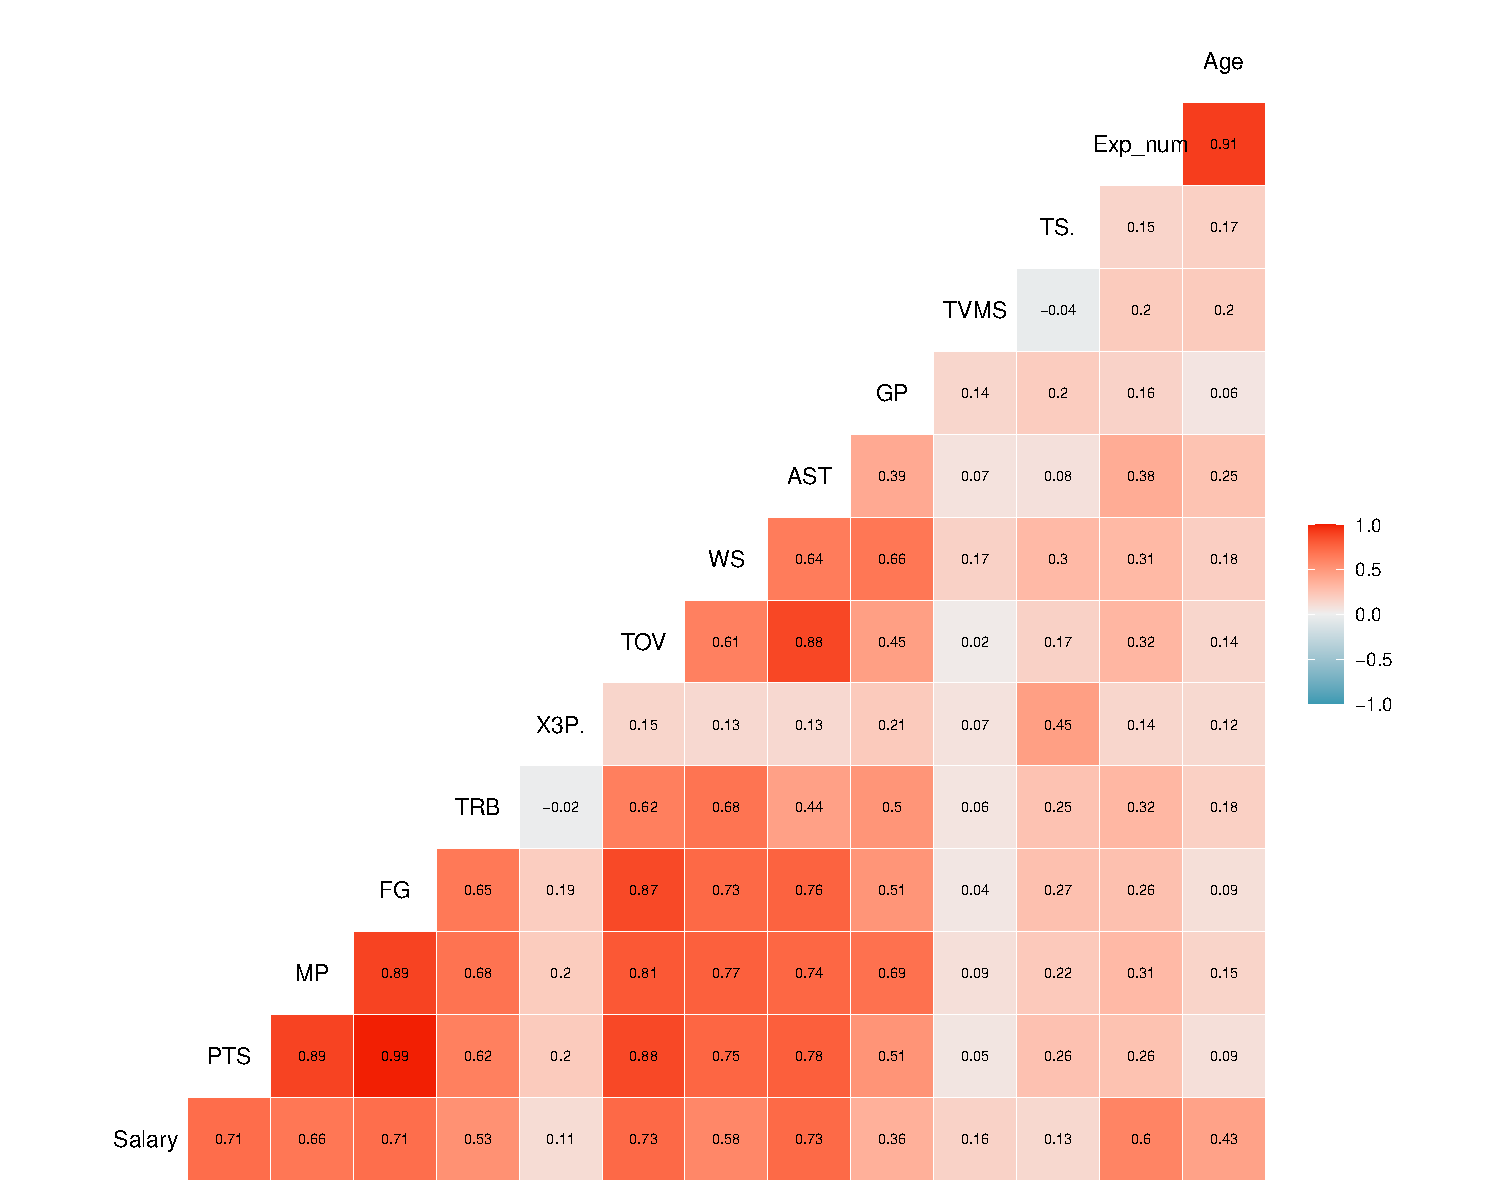
\includegraphics{lab2_report_short_files/figure-latex/corr-plot-1.pdf}
\FloatBarrier

\hypertarget{tab:appendix-vif}{%
\subsection{Collinearity Diagnostics: VIF Comparison}\label{tab:appendix-vif}}

\begin{table}[!h]
\centering
\caption{\label{tab:appendix-vif-table}VIF Comparison Across Models (Excluding Models 1, 4, and 7)}
\centering
\begin{tabular}[t]{lrrrrrr}
\toprule
Variable & Model 2 & Model 3 & Model 5 & Model 6 & Model 8 & Model 9\\
\midrule
PTS & 3.30 & 3.41 & 3.30 & 3.41 & 3.30 & 3.41\\
TRB & 1.63 & 1.73 & 1.63 & 1.73 & 1.63 & 1.73\\
AST & 2.54 & 2.83 & 2.54 & 2.83 & 2.54 & 2.83\\
Exp\_num & NA & 1.29 & NA & 1.29 & NA & 1.29\\
TVMS & NA & 1.04 & NA & 1.04 & NA & 1.04\\
\bottomrule
\end{tabular}
\end{table}
\FloatBarrier

\hypertarget{fig:appendix-hetero}{%
\subsection{Residual Diagnostics for Heteroscedasticity}\label{fig:appendix-hetero}}

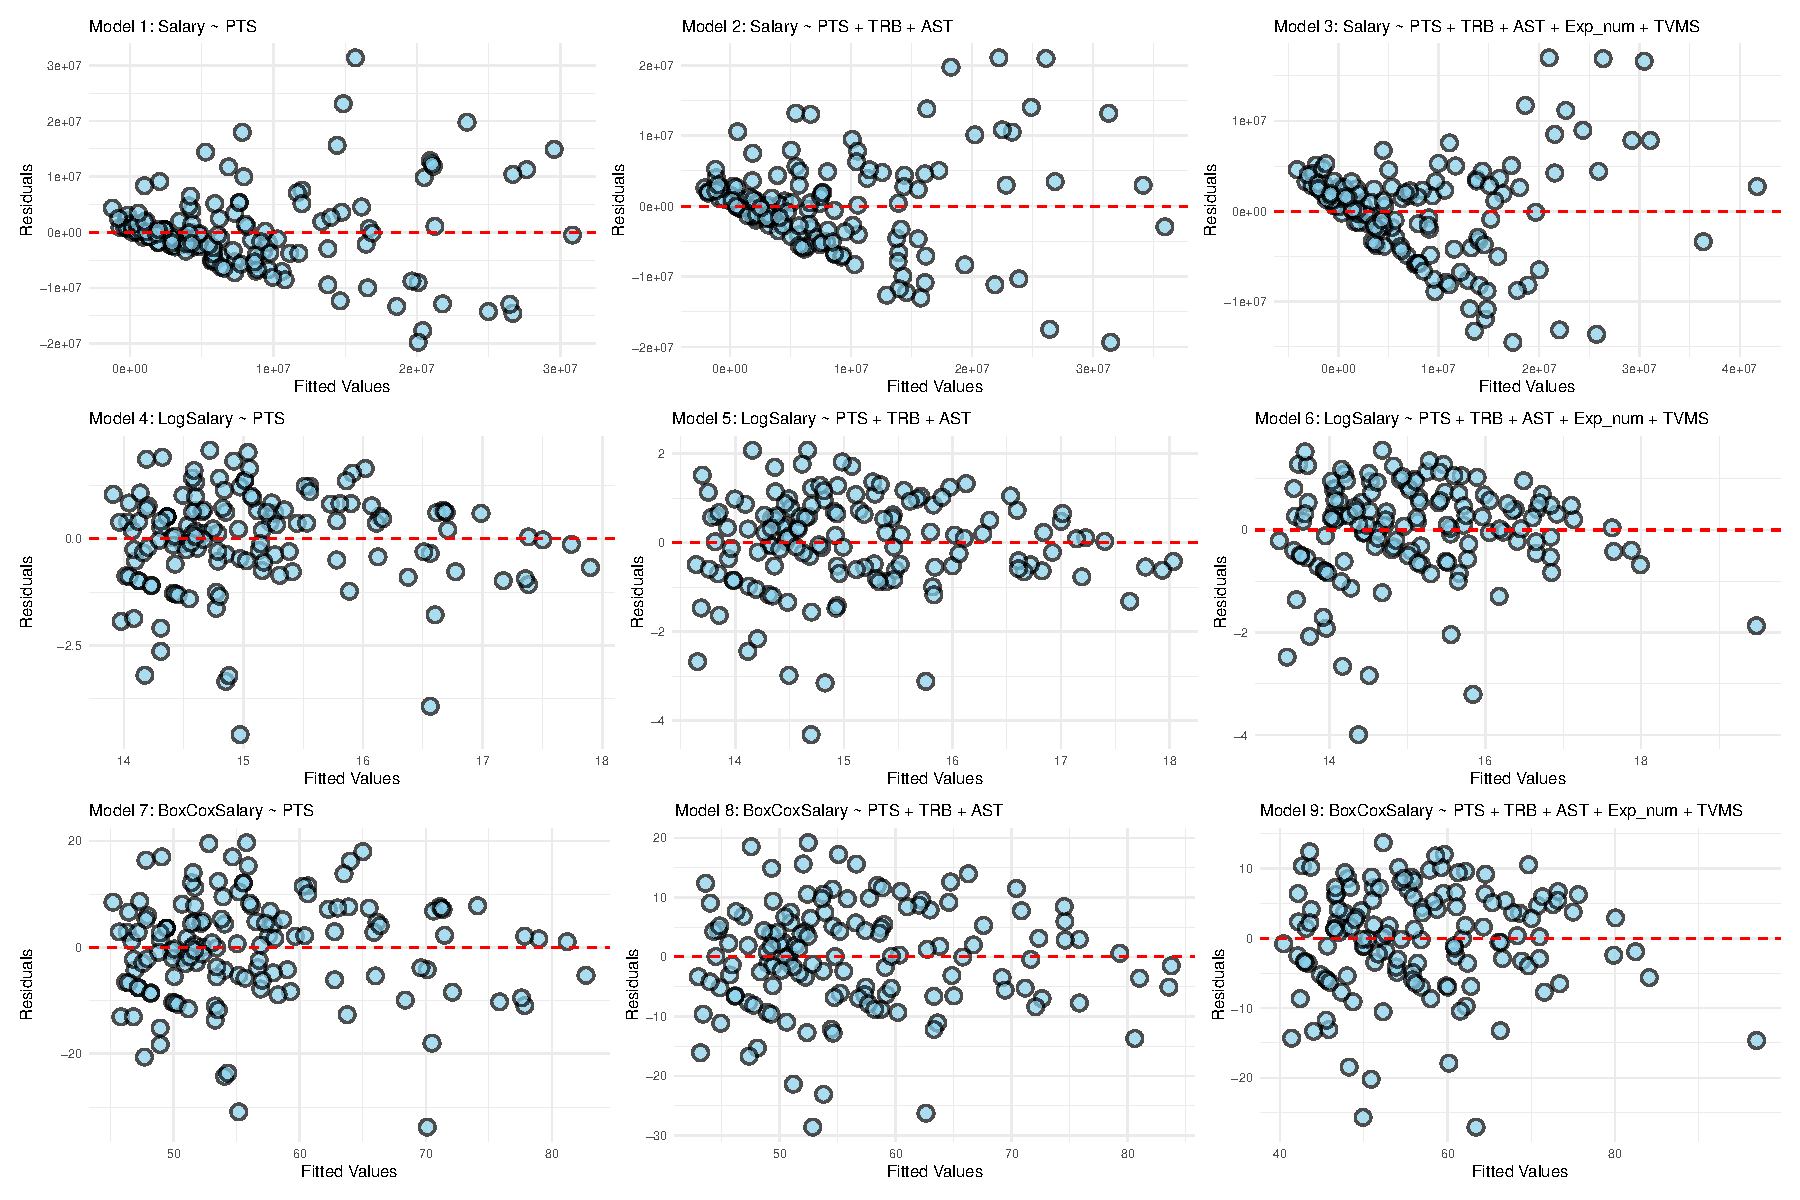
\includegraphics{lab2_report_short_files/figure-latex/appendix-hetero-plot-1.pdf}
\FloatBarrier

\hypertarget{tab:appendix-bp}{%
\subsection{Breusch--Pagan Test Results}\label{tab:appendix-bp}}

\begin{table}[!h]
\centering
\caption{\label{tab:bp-test}Breusch-Pagan Test Results for Heteroscedasticity}
\centering
\begin{tabular}[t]{lrrl}
\toprule
Model & BP Statistic & P-Value & Conclusion\\
\midrule
Model 1 & 31.826 & 0.0000 & Heteroscedastic\\
Model 2 & 53.128 & 0.0000 & Heteroscedastic\\
Model 3 & 47.785 & 0.0000 & Heteroscedastic\\
Model 4 & 0.274 & 0.6006 & Homoscedastic\\
Model 5 & 7.171 & 0.0667 & Homoscedastic\\
\addlinespace
Model 6 & 6.457 & 0.2642 & Homoscedastic\\
Model 7 & 0.284 & 0.5938 & Homoscedastic\\
Model 8 & 7.392 & 0.0604 & Homoscedastic\\
Model 9 & 6.957 & 0.2239 & Homoscedastic\\
\bottomrule
\end{tabular}
\end{table}
\FloatBarrier

\hypertarget{fig:appendix-salary-predictors}{%
\subsection{Salary vs.~Key Predictors}\label{fig:appendix-salary-predictors}}

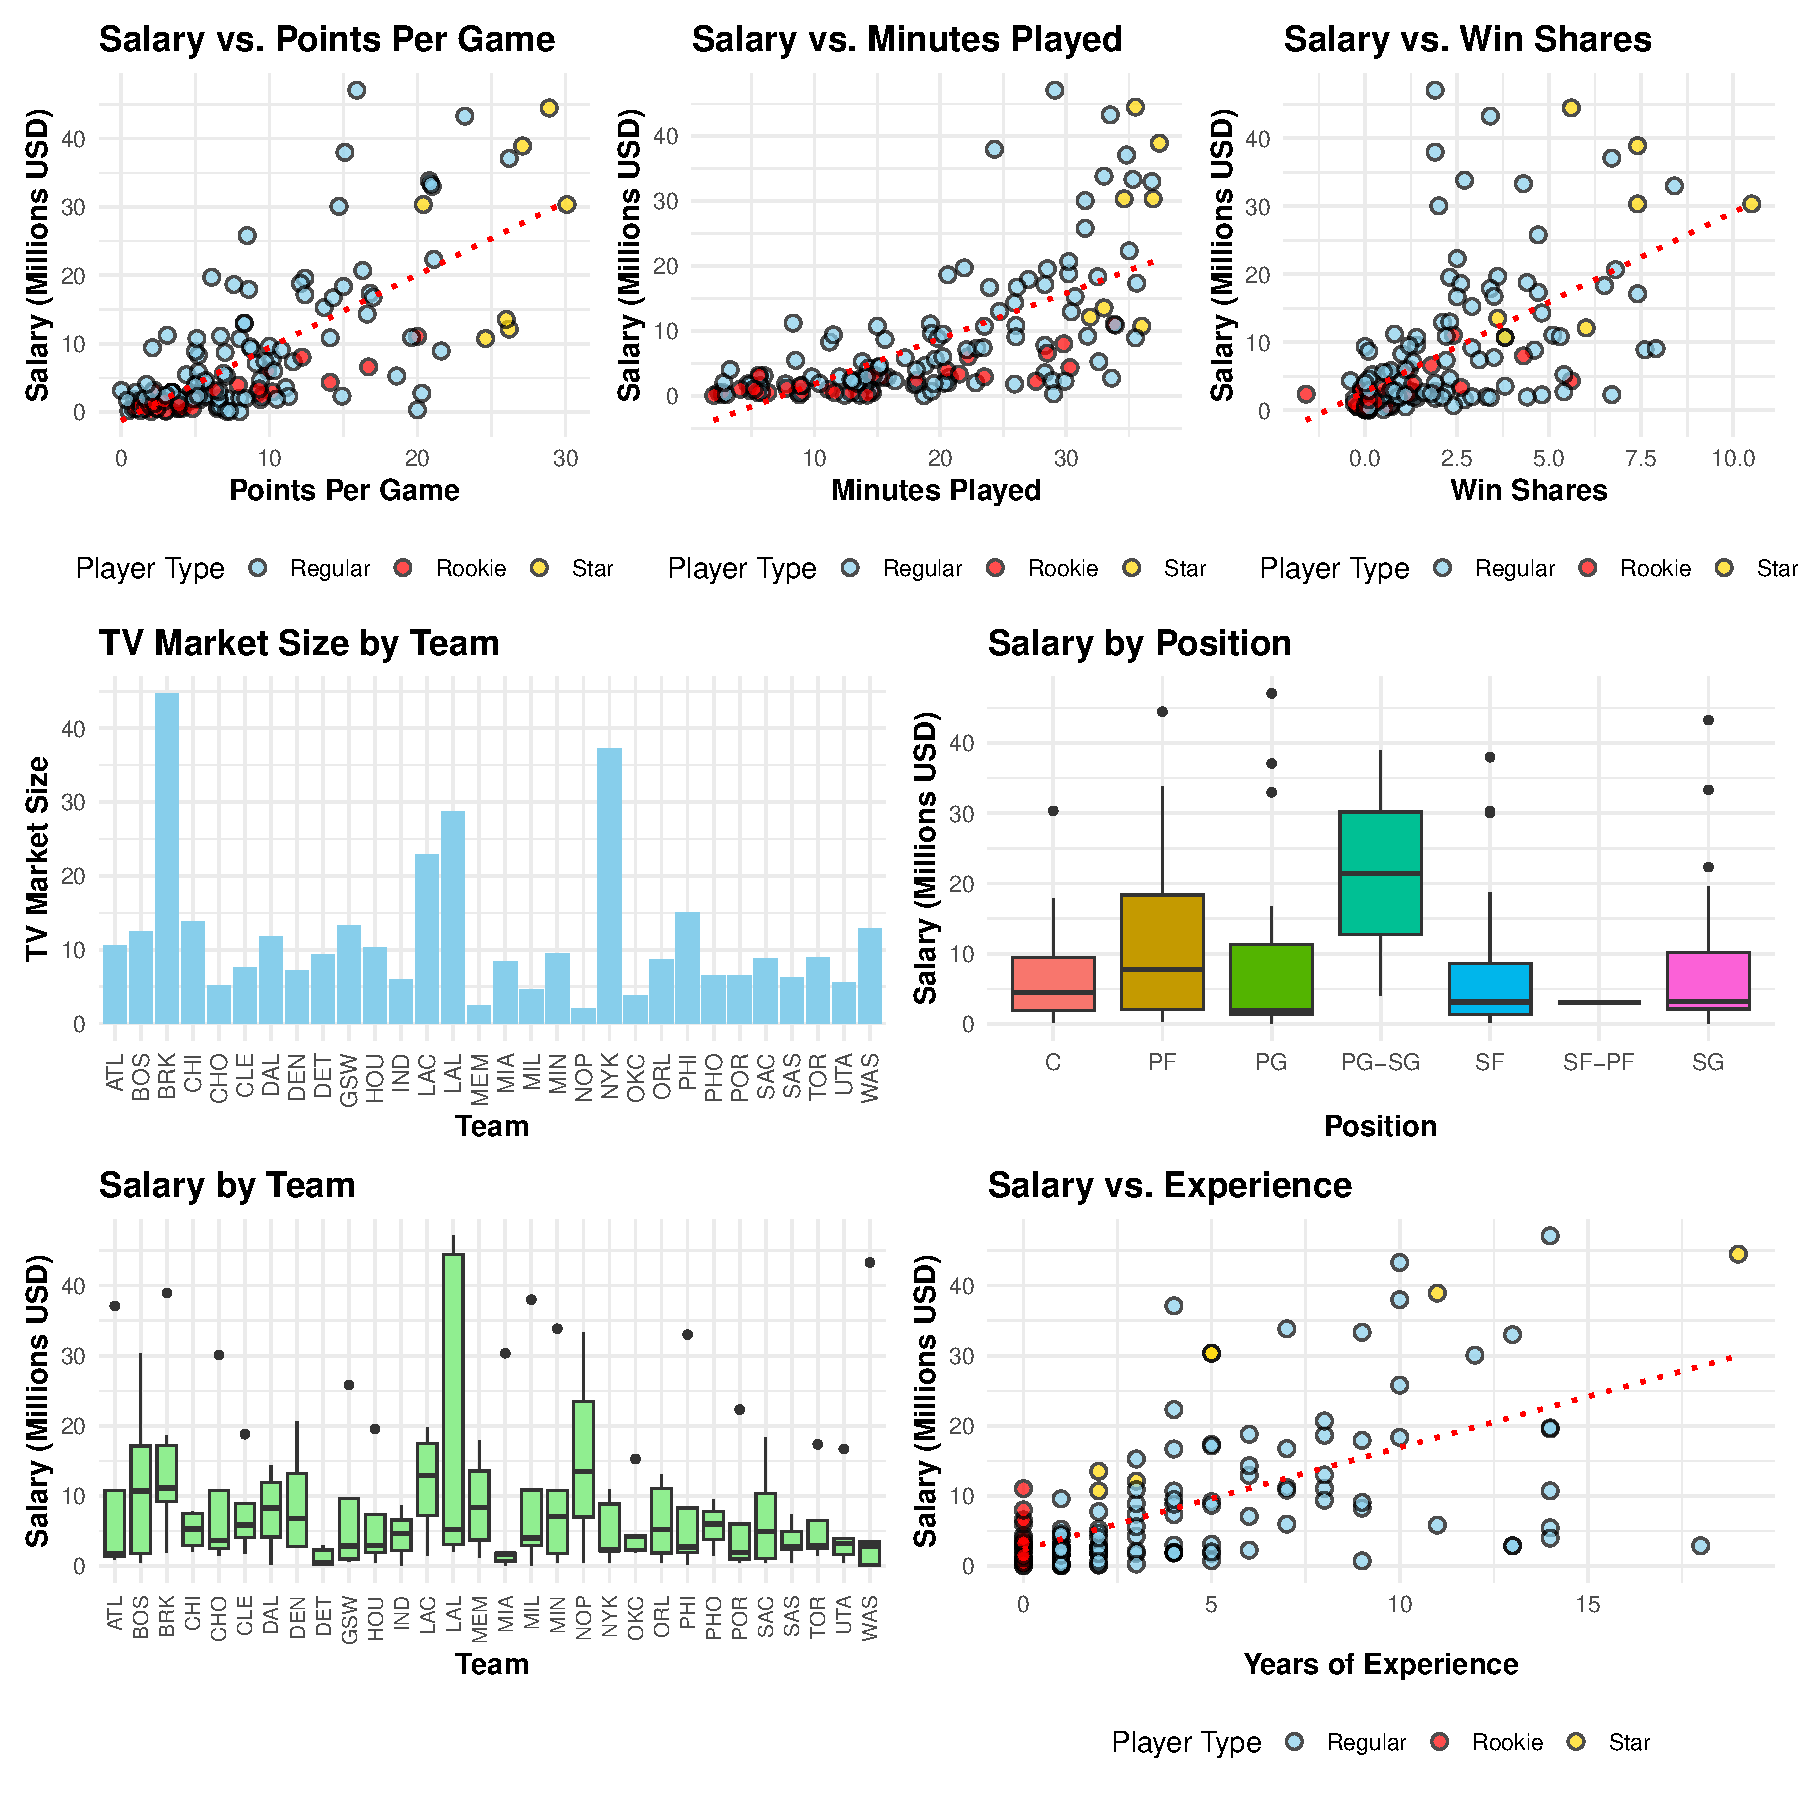
\includegraphics{lab2_report_short_files/figure-latex/salary-predictors-1.pdf}
\FloatBarrier
\newpage

\hypertarget{tab:appendix-models1}{%
\subsection{Raw‐Salary Exploratory Models}\label{tab:appendix-models1}}

\begin{table}[!htbp] \centering 
  \caption{NBA Salary preliminary Models (Raw Salary)} 
  \label{tab:models1} 
\small 
\begin{tabular}{@{\extracolsep{5pt}}lD{.}{.}{-3} D{.}{.}{-3} D{.}{.}{-3} } 
\\[-1.8ex]\hline 
\hline \\[-1.8ex] 
 & \multicolumn{3}{c}{\textit{Dependent variable:}} \\ 
\cline{2-4} 
\\[-1.8ex] & \multicolumn{3}{c}{Salary} \\ 
 & \multicolumn{1}{c}{Model 1} & \multicolumn{1}{c}{Model 2} & \multicolumn{1}{c}{Model 3} \\ 
\hline \\[-1.8ex] 
 PTS & 1,065,213.000^{***} & 371,271.300^{**} & 536,860.500^{***} \\ 
  & (89,908.840) & (147,836.500) & (127,087.400) \\ 
  TRB &  & 816,232.800^{**} & 313,391.500 \\ 
  &  & (325,873.700) & (283,988.600) \\ 
  AST &  & 2,401,759.000^{***} & 1,444,860.000^{***} \\ 
  &  & (454,548.400) & (405,766.900) \\ 
  Exp$_{\text{num}}$ &  &  & 902,796.800^{***} \\ 
  &  &  & (126,761.900) \\ 
  TVMS &  &  & 242,708.300 \\ 
  &  &  & (261,655.200) \\ 
  Constant & -1,226,388.000 & -2,545,865.000^{**} & -4,754,681.000^{***} \\ 
  & (1,024,934.000) & (1,064,685.000) & (1,085,961.000) \\ 
 \hline \\[-1.8ex] 
Observations & \multicolumn{1}{c}{140} & \multicolumn{1}{c}{140} & \multicolumn{1}{c}{140} \\ 
R$^{2}$ & \multicolumn{1}{c}{0.504} & \multicolumn{1}{c}{0.600} & \multicolumn{1}{c}{0.718} \\ 
Adjusted R$^{2}$ & \multicolumn{1}{c}{0.501} & \multicolumn{1}{c}{0.591} & \multicolumn{1}{c}{0.707} \\ 
Residual Std. Error & \multicolumn{1}{c}{7,409,796.000 (df = 138)} & \multicolumn{1}{c}{6,706,668.000 (df = 136)} & \multicolumn{1}{c}{5,673,890.000 (df = 134)} \\ 
F Statistic & \multicolumn{1}{c}{140.368$^{***}$ (df = 1; 138)} & \multicolumn{1}{c}{67.932$^{***}$ (df = 3; 136)} & \multicolumn{1}{c}{68.151$^{***}$ (df = 5; 134)} \\ 
\hline 
\hline \\[-1.8ex] 
\textit{Note:}  & \multicolumn{3}{r}{$^{*}$p$<$0.1; $^{**}$p$<$0.05; $^{***}$p$<$0.01} \\ 
\end{tabular} 
\end{table} 
\FloatBarrier
\newpage

\hypertarget{tab:appendix-models2}{%
\subsection{Log‐Salary Exploratory Models}\label{tab:appendix-models2}}

\begin{table}[!htbp] \centering 
  \caption{NBA Salary preliminary Models (Log Salary)} 
  \label{tab:models2} 
\small 
\begin{tabular}{@{\extracolsep{5pt}}lD{.}{.}{-3} D{.}{.}{-3} D{.}{.}{-3} } 
\\[-1.8ex]\hline 
\hline \\[-1.8ex] 
 & \multicolumn{3}{c}{\textit{Dependent variable:}} \\ 
\cline{2-4} 
\\[-1.8ex] & \multicolumn{3}{c}{LogSalary} \\ 
 & \multicolumn{1}{c}{Model 4} & \multicolumn{1}{c}{Model 5} & \multicolumn{1}{c}{Model 6} \\ 
\hline \\[-1.8ex] 
 PTS & 0.133^{***} & 0.047^{*} & 0.069^{***} \\ 
  & (0.014) & (0.024) & (0.022) \\ 
  TRB &  & 0.219^{***} & 0.150^{***} \\ 
  &  & (0.053) & (0.049) \\ 
  AST &  & 0.192^{**} & 0.061 \\ 
  &  & (0.074) & (0.070) \\ 
  Exp$_{\text{num}}$ &  &  & 0.124^{***} \\ 
  &  &  & (0.022) \\ 
  TVMS &  &  & 0.039 \\ 
  &  &  & (0.045) \\ 
  Constant & 13.911^{***} & 13.559^{***} & 13.244^{***} \\ 
  & (0.162) & (0.173) & (0.187) \\ 
 \hline \\[-1.8ex] 
Observations & \multicolumn{1}{c}{140} & \multicolumn{1}{c}{140} & \multicolumn{1}{c}{140} \\ 
R$^{2}$ & \multicolumn{1}{c}{0.387} & \multicolumn{1}{c}{0.474} & \multicolumn{1}{c}{0.585} \\ 
Adjusted R$^{2}$ & \multicolumn{1}{c}{0.383} & \multicolumn{1}{c}{0.462} & \multicolumn{1}{c}{0.569} \\ 
Residual Std. Error & \multicolumn{1}{c}{1.170 (df = 138)} & \multicolumn{1}{c}{1.092 (df = 136)} & \multicolumn{1}{c}{0.977 (df = 134)} \\ 
F Statistic & \multicolumn{1}{c}{87.166$^{***}$ (df = 1; 138)} & \multicolumn{1}{c}{40.775$^{***}$ (df = 3; 136)} & \multicolumn{1}{c}{37.716$^{***}$ (df = 5; 134)} \\ 
\hline 
\hline \\[-1.8ex] 
\textit{Note:}  & \multicolumn{3}{r}{$^{*}$p$<$0.1; $^{**}$p$<$0.05; $^{***}$p$<$0.01} \\ 
\end{tabular} 
\end{table} 
\FloatBarrier
\newpage

\hypertarget{tab:appendix-models3}{%
\subsection{Box-Cox-Salary Exploratory Models}\label{tab:appendix-models3}}

\begin{table}[!htbp] \centering 
  \caption{NBA Salary preliminary Models (Box-Cox Salary)} 
  \label{tab:models3} 
\small 
\begin{tabular}{@{\extracolsep{5pt}}lD{.}{.}{-3} D{.}{.}{-3} D{.}{.}{-3} } 
\\[-1.8ex]\hline 
\hline \\[-1.8ex] 
 & \multicolumn{3}{c}{\textit{Dependent variable:}} \\ 
\cline{2-4} 
\\[-1.8ex] & \multicolumn{3}{c}{BoxCoxSalary} \\ 
 & \multicolumn{1}{c}{Model 7} & \multicolumn{1}{c}{Model 8} & \multicolumn{1}{c}{Model 9} \\ 
\hline \\[-1.8ex] 
 PTS & 1.245^{***} & 0.461^{**} & 0.669^{***} \\ 
  & (0.118) & (0.198) & (0.174) \\ 
  TRB &  & 1.828^{***} & 1.197^{***} \\ 
  &  & (0.436) & (0.389) \\ 
  AST &  & 1.913^{***} & 0.712 \\ 
  &  & (0.608) & (0.556) \\ 
  Exp$_{\text{num}}$ &  &  & 1.131^{***} \\ 
  &  &  & (0.174) \\ 
  TVMS &  &  & 0.323 \\ 
  &  &  & (0.358) \\ 
  Constant & 45.203^{***} & 42.265^{***} & 39.453^{***} \\ 
  & (1.343) & (1.423) & (1.487) \\ 
 \hline \\[-1.8ex] 
Observations & \multicolumn{1}{c}{140} & \multicolumn{1}{c}{140} & \multicolumn{1}{c}{140} \\ 
R$^{2}$ & \multicolumn{1}{c}{0.448} & \multicolumn{1}{c}{0.536} & \multicolumn{1}{c}{0.656} \\ 
Adjusted R$^{2}$ & \multicolumn{1}{c}{0.444} & \multicolumn{1}{c}{0.525} & \multicolumn{1}{c}{0.644} \\ 
Residual Std. Error & \multicolumn{1}{c}{9.706 (df = 138)} & \multicolumn{1}{c}{8.965 (df = 136)} & \multicolumn{1}{c}{7.768 (df = 134)} \\ 
F Statistic & \multicolumn{1}{c}{111.830$^{***}$ (df = 1; 138)} & \multicolumn{1}{c}{52.273$^{***}$ (df = 3; 136)} & \multicolumn{1}{c}{51.199$^{***}$ (df = 5; 134)} \\ 
\hline 
\hline \\[-1.8ex] 
\textit{Note:}  & \multicolumn{3}{r}{$^{*}$p$<$0.1; $^{**}$p$<$0.05; $^{***}$p$<$0.01} \\ 
\end{tabular} 
\end{table} 
\FloatBarrier
\newpage

\hypertarget{tab:appendix-models-robust}{%
\subsection{Robust SE for Selected Models}\label{tab:appendix-models-robust}}

\begin{table}[!htbp] \centering 
  \caption{NBA Salary Models with Robust Standard Errors} 
  \label{tab:models_robust} 
\small 
\begin{tabular}{@{\extracolsep{5pt}}lD{.}{.}{-3} D{.}{.}{-3} D{.}{.}{-3} } 
\\[-1.8ex]\hline 
\hline \\[-1.8ex] 
 & \multicolumn{3}{c}{\textit{Dependent variable:}} \\ 
\cline{2-4} 
\\[-1.8ex] & \multicolumn{1}{c}{Salary} & \multicolumn{1}{c}{LogSalary} & \multicolumn{1}{c}{BoxCoxSalary} \\ 
 & \multicolumn{1}{c}{Model 3} & \multicolumn{1}{c}{Model 6} & \multicolumn{1}{c}{Model 9} \\ 
\hline \\[-1.8ex] 
 PTS & 536,860.500^{***} & 0.069^{***} & 0.669^{***} \\ 
  & (165,364.900) & (0.023) & (0.200) \\ 
  TRB & 313,391.500 & 0.150^{***} & 1.197^{***} \\ 
  & (320,133.600) & (0.039) & (0.334) \\ 
  AST & 1,444,860.000^{**} & 0.061 & 0.712 \\ 
  & (597,919.800) & (0.063) & (0.558) \\ 
  Exp$_{\text{num}}$ & 902,796.800^{***} & 0.124^{***} & 1.131^{***} \\ 
  & (183,344.700) & (0.021) & (0.188) \\ 
  TVMS & 242,708.300 & 0.039 & 0.323 \\ 
  & (297,389.300) & (0.037) & (0.324) \\ 
  Constant & -4,754,681.000^{***} & 13.244^{***} & 39.453^{***} \\ 
  & (997,226.400) & (0.219) & (1.626) \\ 
 \hline \\[-1.8ex] 
Robust p-val: PTS & 0.001 & 0.003 & 0.001 \\ 
Robust p-val: TRB & 0.329 & 0 & 0 \\ 
Robust p-val: AST & 0.017 & 0.339 & 0.204 \\ 
Robust p-val: Exp$_{\text{num}}$ & 0 & 0 & 0 \\ 
Robust p-val: TVMS & 0.416 & 0.29 & 0.321 \\ 
Observations & \multicolumn{1}{c}{140} & \multicolumn{1}{c}{140} & \multicolumn{1}{c}{140} \\ 
R$^{2}$ & \multicolumn{1}{c}{0.718} & \multicolumn{1}{c}{0.585} & \multicolumn{1}{c}{0.656} \\ 
Adjusted R$^{2}$ & \multicolumn{1}{c}{0.707} & \multicolumn{1}{c}{0.569} & \multicolumn{1}{c}{0.644} \\ 
Residual Std. Error (df = 134) & \multicolumn{1}{c}{5,673,890.000} & \multicolumn{1}{c}{0.977} & \multicolumn{1}{c}{7.768} \\ 
F Statistic (df = 5; 134) & \multicolumn{1}{c}{68.151$^{***}$} & \multicolumn{1}{c}{37.716$^{***}$} & \multicolumn{1}{c}{51.199$^{***}$} \\ 
\hline 
\hline \\[-1.8ex] 
\textit{Note:}  & \multicolumn{3}{r}{$^{*}$p$<$0.1; $^{**}$p$<$0.05; $^{***}$p$<$0.01} \\ 
\end{tabular} 
\end{table} 
\FloatBarrier
\newpage

\hypertarget{data-dictionary} & 3-point shooting percentage\tabularnewline
TOV & Turnovers per game\tabularnewline
WS & Win shares\tabularnewline
GP & Games played\tabularnewline
AST & Assists per game\tabularnewline
TVMS & TV Market Size\tabularnewline
TS\% & True Shooting Percentage\tabularnewline
star\_player & All-Star status (1=Yes, 0=No)\tabularnewline
Position & Player position\tabularnewline
Age & Player age\tabularnewline
Exp\_num & Years of NBA experience\tabularnewline
\bottomrule
\end{longtable}

\hypertarget{references}{%
\section{References}\label{references}}

\begin{enumerate}
\def\labelenumi{\arabic{enumi}.}
\item
  Southwest Journal. (n.d.). \emph{NBA Players' Salaries: How Much Do NBA Players Make?} Retrieved from \url{https://www.southwestjournal.com/sport/nba/nba-players-salaries/?utm_source=chatgpt.com}
\item
  Papadaki, I., \& Tsagris, M. (2020). \emph{Are NBA Players' Salaries in Accordance with Their Performance on Court?} In \emph{Advances in Econometrics, Operational Research, Data Science and Actuarial Studies} (pp.~405--428). \url{https://doi.org/10.1007/978-3-030-85254-2_25}
\item
  Sigler, K.J., \& Sackley, W.H. (2000). \emph{NBA Players: Are They Paid for Performance?} \emph{Managerial Finance, 26}(7), 46--51. \url{https://doi.org/10.1108/03074350010766783}
\item
  Bautista, M., Khorobrykh, K., Platz, T., \& Lin, DW. (2024). NBA Salary and Performance: Exploratory Data Analysis {[}R~Markdown file{]}. GitHub repository. Retrieved April~17,~2025, from \url{https://github.com/mids-w203/lab-2-pacific-boys-1/blob/main/notebooks/analysis_lab2_short/lab2_report_short.Rmd}
\end{enumerate}

\end{document}
